%%%%%%%%%%%%%%%%%%%%%%%%%%%%%%%%%%%%%%%%%%%%%%%%%%%%%%%%%%%%%%%%%%%%%%
% LaTeX Example: Project Report
%
% Source: http://www.howtotex.com
%
% Feel free to distribute this example, but please keep the referral
% to howtotex.com
% Date: March 2011 
% 
%%%%%%%%%%%%%%%%%%%%%%%%%%%%%%%%%%%%%%%%%%%%%%%%%%%%%%%%%%%%%%%%%%%%%%
% How to use writeLaTeX: 
%
% You edit the source code here on the left, and the preview on the
% right shows you the result within a few seconds.
%
% Bookmark this page and share the URL with your co-authors. They can
% edit at the same time!
%
% You can upload figures, bibliographies, custom classes and
% styles using the files menu.
%
% If you're new to LaTeX, the wikibook is a great place to start:
% http://en.wikibooks.org/wiki/LaTeX
%
%%%%%%%%%%%%%%%%%%%%%%%%%%%%%%%%%%%%%%%%%%%%%%%%%%%%%%%%%%%%%%%%%%%%%%
% Edit the title below to update the display in My Documents
%\title{Project Report}
%
%%% Preamble
\documentclass[paper=a4, fontsize=11pt]{scrartcl}
\usepackage[T1]{fontenc}
\usepackage{fourier}
\usepackage{abstract}
\usepackage[english]{babel}															% English language/hyphenation
\usepackage[protrusion=true,expansion=true]{microtype}	
\usepackage{amsmath,amsfonts,amsthm} % Math packages
\usepackage[pdftex]{graphicx}	
\usepackage{url}
\usepackage{float}


%%% Custom sectioning
\usepackage{sectsty}
\allsectionsfont{\centering \normalfont\scshape}


%%% Custom headers/footers (fancyhdr package)
\usepackage{fancyhdr}
\pagestyle{fancyplain}
\fancyhead{}											% No page header
\fancyfoot[L]{}											% Empty 
\fancyfoot[C]{}											% Empty
\fancyfoot[R]{\thepage}									% Pagenumbering
\renewcommand{\headrulewidth}{0pt}			% Remove header underlines
\renewcommand{\footrulewidth}{0pt}				% Remove footer underlines
\setlength{\headheight}{13.6pt}


%%% Equation and float numbering
\numberwithin{equation}{section}		% Equationnumbering: section.eq#
\numberwithin{figure}{section}			% Figurenumbering: section.fig#
\numberwithin{table}{section}				% Tablenumbering: section.tab#


%%% Maketitle metadata
\newcommand{\horrule}[1]{\rule{\linewidth}{#1}} 	% Horizontal rule

\title{
		%\vspace{-1in} 	
		\usefont{OT1}{bch}{b}{n}
		\normalfont \normalsize \textsc{Autonomous Agents Assignment 1} \\ [25pt]
		\horrule{0.5pt} \\[0.4cm]
		\huge Single Agent Planning \\
		\horrule{2pt} \\[0.5cm]
}
\author{
		%\normalfont 								\normalsize
        Duy Chuan Ha, Said Al Faraby, Christos Louizos, Oana Munteanu %[-3pt]		%\normalsize
        \\
        \\
        \today
}
\date{}
\renewcommand{\abstractnamefont}{\normalfont\Large\bfseries}
\renewcommand{\abstracttextfont}{\normalfont\bfseries}


%%% Begin document
\begin{document}
\maketitle
\bigskip
\bigskip
\bigskip
\bigskip
\begin{abstract}
%change first sentence
The aim of this assignment is to make a research according to the planning scenario in which the main goal of the predator is to capture the prey.\\ 
The report comprises the methods that have been implemented by using the Dynamic Programming paradigm, namely policy evaluation, policy iteration and value iteration. Our contribution on Single Agent Planning reveals the comparison between the implemented methods in terms of convergence time and results. \\ +Conclusion
\end{abstract}
\newpage
\tableofcontents 
\newpage

\section{Introduction}
We begin the following report by first explaining the predator-prey environment and defining it's goal in section~\ref{environment}. Afterwards we present in section~\ref{methods} the various methods that were implemented in the afforementioned environment. The results that derived from each of these methods are displayed in detail in section~\ref{results} and finally there is a discussion as well as a comparison between them in section~\ref{discussion}

\subsection{Environment}
\label{environment}
The environment is encoded as a state of two positions, the one of the predator and the prey. 
%insert later dataflow diagram
The simulator is defined through a while-loop of a hundred runs where the initial position of the predator is (0,0) and that of the prey (5,5). In each transition, the predator will make a move first and then the prey, according to their respective policies. Each run can be "seen" as an episode where the goal of the predator is to capture the prey, which can be interpreted as the end state of this particular episode. 

Both the predator and the prey are initialized with a random policy in the beginning where for the predator it is equiprobable to choose any of the possible actions %$\alpha \in A\{\textit{north, south, east, west, wait}\}$ 
in any state. The prey has a steady policy and hence it can be modeled as part of the environment. It has 0.8 probability of waiting at any given state and 0.2 probability of moving to any of the adjacent squares.

\section{Methods and Procedures}
\label{methods}
\subsection{Implementation overview}
\begin{figure}[H] \centering
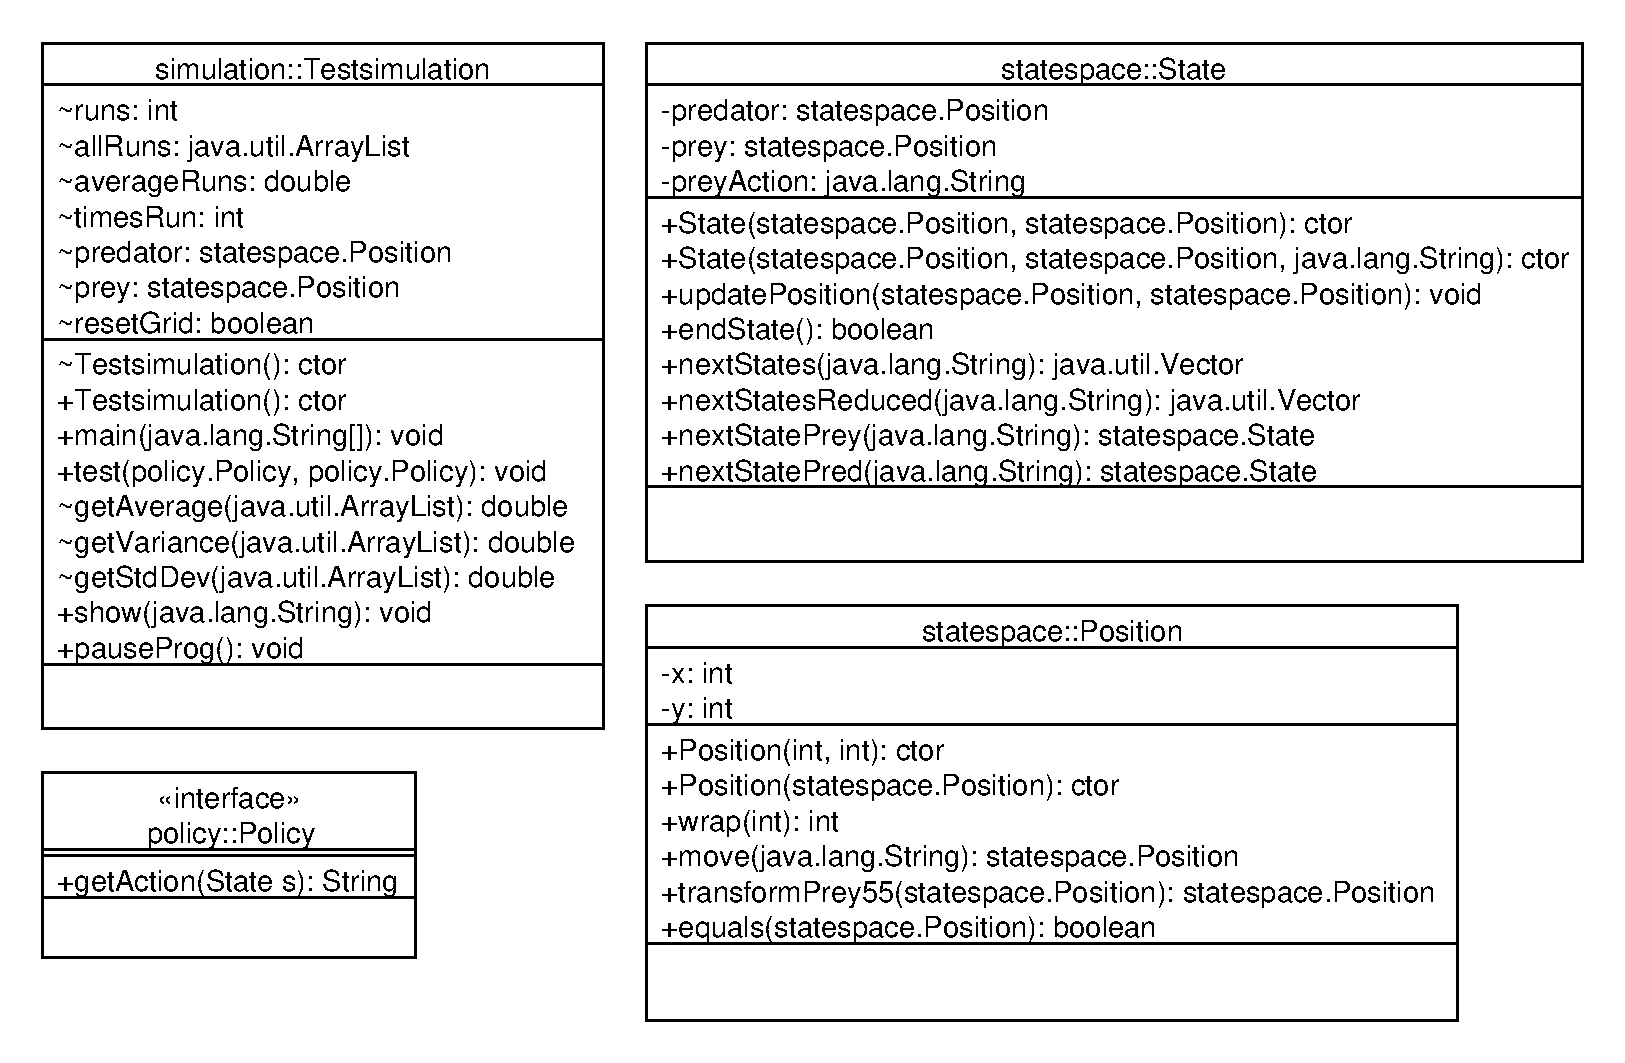
\includegraphics[scale=0.6]{uml_general.pdf}
\caption{Predator-prey domain framework} \label{Predator-prey domain framework}
\end{figure}
\begin{figure}[H] \centering
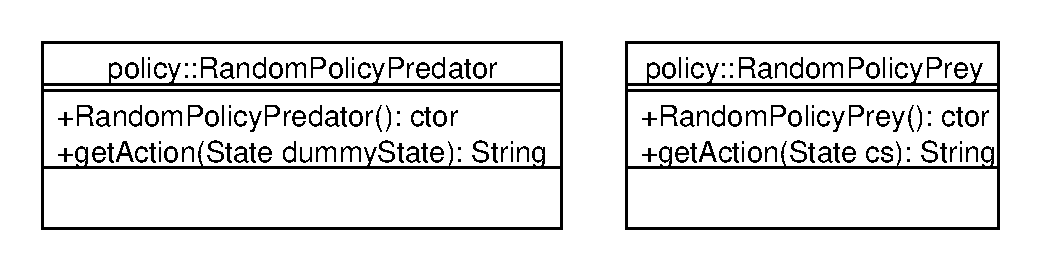
\includegraphics[scale=0.6]{uml_policies1.pdf}
\caption{Random policies implemented} \label{Policies1}
\end{figure}
\begin{figure}[H] \centering
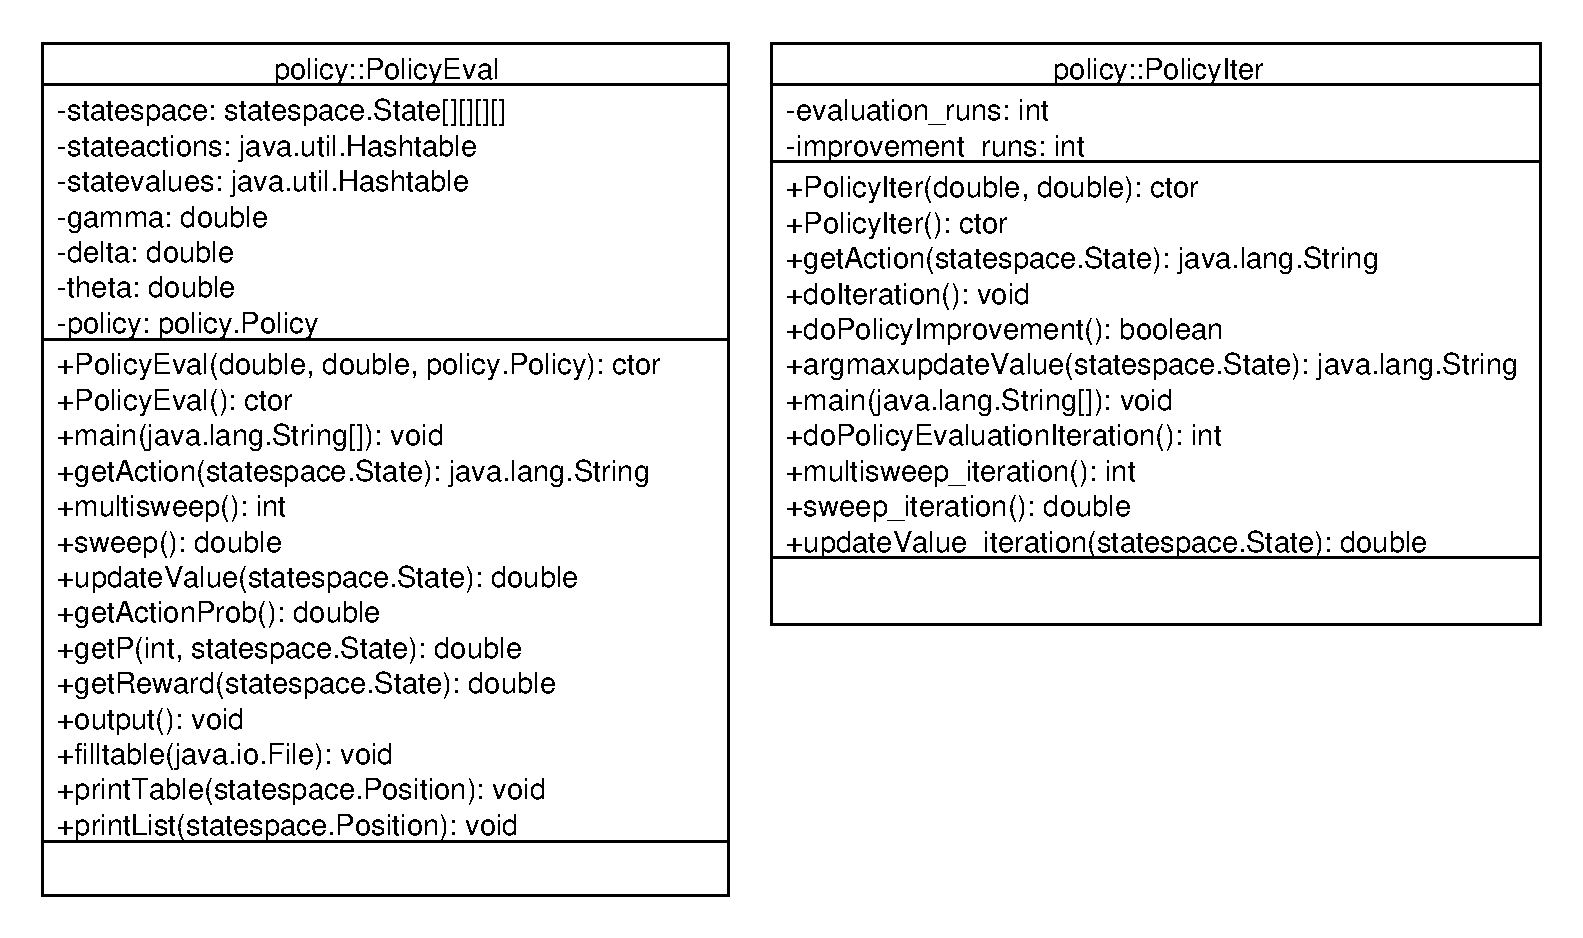
\includegraphics[scale=0.6]{uml_policies2.pdf}
\caption{Policy evaluation and iteration implemented} \label{Policies2}
\end{figure}
\begin{figure}[H] \centering
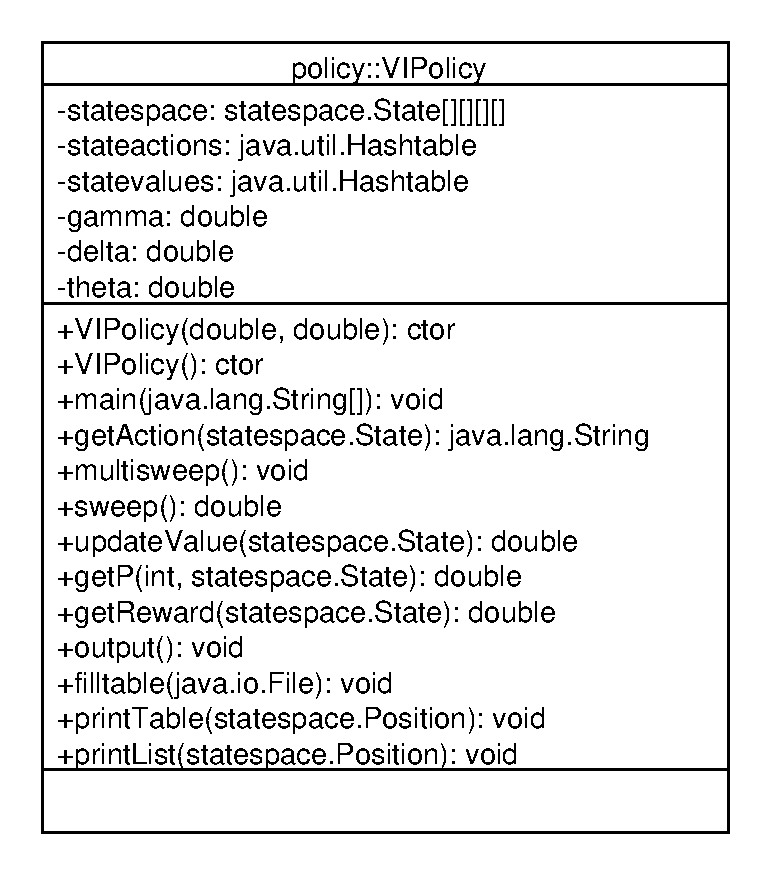
\includegraphics[scale=0.58]{uml_policies3.pdf}
\caption{Policy value iteration implemented} \label{Policies3}
\end{figure}

\subsection{Iterative Policy Evaluation}
In Marcov Decision Processes, one of the important steps is evaluation step, which is to find the state-value functions $V^\pi$ for an arbitrary policy, $\pi$. The state-value functions estimate value of a state in terms of expected return that can be obtained from that state. Below is the equation for calculating $V^\pi$.
\begin{align}
V^\pi(s)&=E_\pi\left\lbrace r_{t+1}+\gamma V^\pi(s_{s+1})\mid s_t=s \right\rbrace\notag\\
&=\sum_{a}\pi(s,a)\sum_{s'}P_{ss'}^a[R_{ss'}^a+\gamma V^\pi(s')] \label{oriV}
\end{align}
where $\mathbf{\pi(s,a)}$ is probability of taking action $\mathbf{a}$ in state $\mathbf{s}$ under policy $\mathbf{\pi}$, $P_{ss'}^a$ is probability of end up at state $\mathbf{s'}$ after taking action $\mathbf{a}$ in state $\mathbf{s}$, $R_{ss'}^a$ is expected immediate reward on transition from $\mathbf{s}$ to $\mathbf{s'}$ under action $\mathbf{a}$, and $\mathbf{\gamma}$ is a discount factor.\\
\\
Since in our test environment the dinamics are completely known, then  equation $\eqref{oriV}$ can be solved using iterative solution methods. By iterative solution methods, we can consider there is a sequence of $V$, $V_0, V_1, V_2, \dots$, each mapping all states in $S^+$ to $\Re$. The initial values of $V^\pi$ are chosen arbitrarily, and the update rule for each successive state-values are gained by following the Bellman equation :
\begin{align}
V_{k+1}(s) &= E_\pi\left\lbrace r_{t+1}+\gamma V_{k}(s_{t+1}\mid s_t=s) \right\rbrace\notag\\
&=\sum_{a}\pi(s,a)\sum_{s'}P_{ss'}^a [R_{ss'}^a+\gamma V_k(s')] \label{iterV}
\end{align}
For the technical implementation, we used one array to save state-values and updated the values in place. This implementation is slightly different from $\eqref{iterV}$, because there is a possibility that $V_k(s')$ uses new values  instead of old ones, but this implementation still guarantees to converge to $V^\pi$. Another technical implementation to be considered is the stopping criteria. In formal, iterative policy iteration will converge only in the limit, but for practical purposes stopping condition is necessary. One of common criteria to stop the sweep is when there is no any single state managed to make a significant changes to their values. A complete pseudocode of the whole processes of the iterative policy evaluation is shown in figure $\ref{Iterative Policy Evaluation Pseudo}$.
\begin{figure}[H] \centering
\fbox{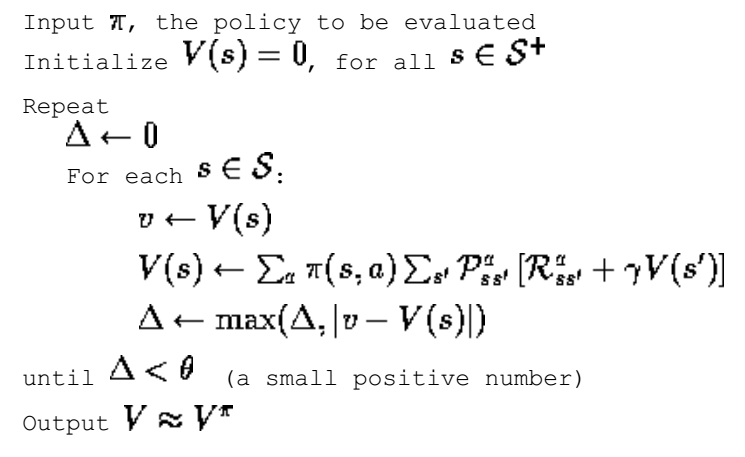
\includegraphics[scale=0.6]{policyIterPseudo.png}}
\caption{Iterative Policy Evaluation} \label{Iterative Policy Evaluation Pseudo}
\end{figure}

\subsection{Policy Iteration}
Policy iteration is composed by two steps, the policy evaluation, which was explained above, and the policy improvement. The main reason for calculating the value function for a policy is to use it in order to find better policies. Consequently if we have determined the value function $V^{\pi}$ for a deterministic policy $\pi$ we can then select a different action $\alpha$ for one state $s$ and afterwards keep on using that specific action for that state, and then continue following the existing policy. Therefore we can determine if the change improved the policy by calculating the following formula:
\begin{align}
Q^\pi(s,\alpha) & = E_\pi \{r_{t+1} + \gamma V^{\pi} (s_{t+1})| s_t = s, \alpha_t = \alpha\}\notag\\
& = \sum_{s'}^{}P_{ss'}^{\alpha}[R_{ss'}^{\alpha}+\gamma V^\pi(s')]
\end{align}
if this is greater than the value of the existing policy in that state $V^\pi(s)$ then it would be better to continue taking action $\alpha$ everytime we encounter state $s$, which results in a new policy $\pi'$. This is true because it derives from the policy improvement theorem where if we have two deterministic policies $\pi$ and $\pi'$ such that for all states $s \in \mathbf{S}$ the $Q^\pi(s,\pi'(s)) >= V^\pi(s)$ then the policy $\pi'$ must be equal to or better than policy $\pi$ meaning that it will yield equal or higher values for all state $s$. Thus if $Q^\pi(s,\alpha) > V^\pi(s)$ then the changed policy $\pi'$ is indeed better than $\pi$. There is one more step needed in order to finish the policy improvement. Since we can acquire a better reward by doing a different action than the one the policy provide at a given state, then it makes sense to choose the action that maximizes that reward and incorporate it to the new policy $\pi'$. Then the formula resulting from this step is:
\begin{align}
\pi'(s) &= arg\max_\alpha Q^\pi(s,\alpha)\notag\\
&= arg\max_\alpha E{r_{t+1} + \gamma V^\pi(s_{t+1})|s_t=s,\alpha_t=\alpha}\notag\\
&= arg\max_\alpha \sum_{s'}P_{ss'}{\alpha}[R_{ss'}^{\alpha} + \gamma V^\pi(s')]
\end{align}
where $arg\max_\alpha$ denotes the action that maximizes the term that is following. Taking all the above into consideration we can say that the process of making a new policy that improves the existing one by being greedy on the value function of the original policy, is called policy improvement.

The whole pseudocode loop of iterative evaluation of the current policy and improvement of the current policy in order to produce a better policy $\pi'$ untill we converge to the optimal policy is illustrated in figure \ref{Policy Iteration}.

\begin{figure}[H] \centering
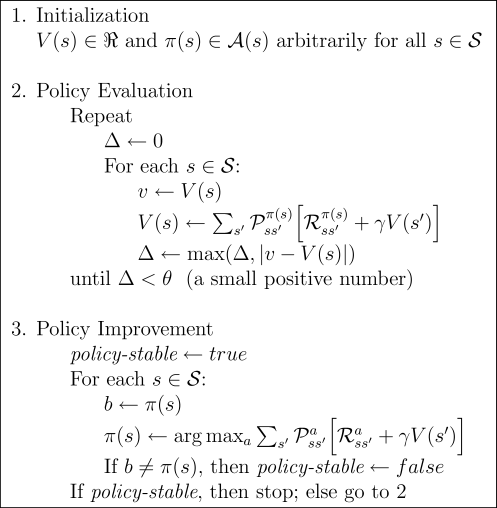
\includegraphics[scale=0.55]{pseudotmp1.png}
\caption{Policy Iteration} \label{Policy Iteration}
\end{figure}

We begin by initializing the values and actions for the policy arbitrarily and afterwards we perform policy evaluation untill the difference in the values are smaller than a certain small threshold $\theta$. After this step we begin the policy improvement step where we find the best possible action for each possible state, with respect to maximizing the value. If the resulting actions are the same as the current policy then we have reached the optimal policy, otherwise we perform policy evaluation again on the new policy and keep on the same procedure untill we converge to the optimal one.

\subsection{Value Iteration}
Value iteration extends on Policy iteration in which the policy evaluation step of policy evaluation is stopped after just one sweep, ie there's one backup of each state. It consists of a backup operation that combines the policy improvement and truncated policy evaluation steps:
\begin{align}
V_{k+1}(s) &= \max_{a} E{r_{t+1} + \gamma V_k(s_{t+1}) | s_t=s, a_t=a}\notag\\
& = \max_{a} \sum_{s'} P_{ss'}^a [R_{ss'}^a + \gamma V_k(s')]
\end{align}
From this we can see it's identical to the Policy evaluation except that it requires the maximum to be taken over all actions. The algorithm, as previous algorithms converge to an optimal policy for discounted finite MPDs. Formally, convergent to $V^{*}$ is only reached when the number of iterations is taken to infinity. In practice we consider $\theta$ as the termination condition of the loop, which keeps track of the change in value funtion. The pseudocode for value iteration is shown in the following figure:
\begin{figure}[H] \centering
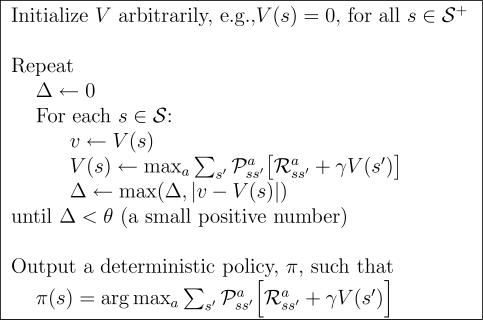
\includegraphics[scale=0.6]{sutton4_5valueiteration.png}
\caption{Value Iteration} \label{Value Iteration}
\end{figure}
As in our implementation of policy evaluation and policy iteration, the backup operation is done "in-place", thus faster convergent is reached. The rate of convergent hereby is very much dependant on the order in which states are backed up during the sweep. In our implementation the order is straightforward; it's aligned with the array[i][j], starting with the x-coordinate $x_i$. From the second row forward the benefit hereby is valued at most $3V_{k}$, leaving at minimum $2V_{k-1}$ still containing the old values, where $k$ denotes the current sweep.

\subsection{Reducing the state space}
\label{reduce}

\section{Results}
\label{results}

\subsection{Random Policy}
\begin{table} [ht]
\caption{Random policy results}
\centering
    \begin{tabular}{| l || l |}
    \hline
     For 100 runs & Summary \\ \hline
    Average time to capture the prey & 336.78\\ \hline
    Standard deviation & 285.66324859876534 \\
    \hline
    \end{tabular}
\end{table}

\subsection{Iterative Policy Evaluation}
The goal of the experiment in this algorithm was to evaluate the arbitrary policy, and to measure the number of iteration it took to converge. There were two parameters should be defined, discount factor $\mathbf{\gamma}$ and a threshold value for stopping condition $\mathbf{\theta}$. The values of the parameters along with some results are shown in the following table.
\begin{table} [ht]
\caption{Policy evaluation results}
\centering
    \begin{tabular}{| l || l |}
    \hline
      & Summary \\ \hline
    $\gamma$ & 0.8 \\ \hline
    $\theta$ & 1.0E-20 \\ \hline
    runtime & 12248712457 ns \\ \hline
    Number of iterations & 106 \\
    \hline
    \end{tabular} \\
\end{table}
Runtime is time that the algorithm took to converge, and it was measured in nanosecond. While the number of iterations is the number of sweep (sweep is backup operation for all states) until it converged.

\begin{table}[ht]
\caption{State values for the following states}
\centering
\begin{tabular}{| l  |  l || c | r |}
  \hline
  Predator & Prey & $V(s)$ \\ \hline
  (0,0) & (5,5) & 0.005724141401102873 \\ \hline
  (2,3) & (5,4) & 0.18195076385152237 \\ \hline
  (2,10) & (10,10) & 0.18195076385152237 \\ \hline
  (10,10) & (10,10) & 1.1945854778368172 \\
  \hline  
\end{tabular}
\end{table}


reduced
nr iteration = 19
Time : 179385026

\subsection{Policy Iteration}
For all the experiments with policy Iterations theta was defined heuristically as $\theta = \exp(-20)$.

\begin{table}[ht]
\caption{Convergence in iterations for different $\gamma$}
\centering
\begin{tabular}{|l||c|c|}
\hline
$\gamma$&Evaluation runs&Improvement runs\\
\hline
0.1&100&8\\
\hline
0.5&227&7\\
\hline
0.7&323&8\\
\hline
0.9&763&10\\
\hline
\end{tabular}
\label{convPIter}
\end{table}

The values for for every possible state when the prey is at [5][5] are illustrated in table~\ref{pitS}
\begin{table}[ht]
\caption{Values from policy iteration when the prey is at [5][5]}
\centering
\begin{tabular}{l*{9}{c}r}
  \hline
3.883 & 4.291 & 4.742 & 5.237 & 5.792 & 6.251 & 5.792 & 5.237 & 4.742 & 4.291 & 3.883  \\
4.291 & 4.712 & 5.228 & 5.802 & 6.436 & 6.997 & 6.436 & 5.802 & 5.228 & 4.712 & 4.291  \\
4.742 & 5.228 & 5.802 & 6.440 & 7.148 & 7.839 & 7.148 & 6.440 & 5.802 & 5.228 & 4.742  \\
5.237 & 5.802 & 6.440 & 7.148 & 7.936 & 8.780 & 7.936 & 7.148 & 6.440 & 5.802 & 5.237  \\
5.792 & 6.436 & 7.148 & 7.936 & 8.780 & 10.000 & 8.780 & 7.936 & 7.148 & 6.436 & 5.792  \\
6.251 & 6.997 & 7.839 & 8.780 & 10.000 & 0.000 & 10.000 & 8.780 & 7.839 & 6.997 & 6.251  \\
5.792 & 6.436 & 7.148 & 7.936 & 8.780 & 10.000 & 8.780 & 7.936 & 7.148 & 6.436 & 5.792  \\
5.237 & 5.802 & 6.440 & 7.148 & 7.936 & 8.780 & 7.936 & 7.148 & 6.440 & 5.802 & 5.237  \\
4.742 & 5.228 & 5.802 & 6.440 & 7.148 & 7.839 & 7.148 & 6.440 & 5.802 & 5.228 & 4.742  \\
4.291 & 4.712 & 5.228 & 5.802 & 6.436 & 6.997 & 6.436 & 5.802 & 5.228 & 4.712 & 4.291  \\
3.883 & 4.291 & 4.742 & 5.237 & 5.792 & 6.251 & 5.792 & 5.237 & 4.742 & 4.291 & 3.883
\end{tabular}
\label{pitS}
\end{table}

\subsection{Value Iteration}

\begin{table}[ht]
\caption{Convergence in iterations for different $\gamma$}
\centering
\begin{tabular}{|l||r|}
\hline
$\gamma$ & Nr. of iterations\\
\hline
0.1& 18\\
\hline
0.5& 25\\
\hline
0.7& 27\\
\hline
0.9& 29\\
\hline
\end{tabular}
\label{convVIter}
\end{table}

The values for for every possible state when the prey is at [5][5] are illustrated in table~\ref{pitS}
\begin{table}[ht]
\caption{Values from value iteration when the prey is at [5][5]}
\centering
\begin{tabular}{l*{9}{c}r}
  \hline
3.883 & 4.291 & 4.742 & 5.237 & 5.792 & 6.251 & 5.792 & 5.237 & 4.742 & 4.291 & 3.883 \\
4.291 & 4.712 & 5.228 & 5.802 & 6.436 & 6.997 & 6.436 & 5.802 & 5.228 & 4.712 & 4.291 \\
4.742 & 5.228 & 5.802 & 6.440 & 7.148 & 7.839 & 7.148 & 6.440 & 5.802 & 5.228 & 4.742 \\
5.237 & 5.802 & 6.440 & 7.148 & 7.936 & 8.780 & 7.936 & 7.148 & 6.440 & 5.802 & 5.237 \\
5.792 & 6.436 & 7.148 & 7.936 & 8.780 & 10.000 & 8.780 & 7.936 & 7.148 & 6.436 & 5.792 \\
6.251 & 6.997 & 7.839 & 8.780 & 10.000 & 0.000 & 10.000 & 8.780 & 7.839 & 6.997 & 6.251 \\
5.792 & 6.436 & 7.148 & 7.936 & 8.780 & 10.000 & 8.780 & 7.936 & 7.148 & 6.436 & 5.792 \\
5.237 & 5.802 & 6.440 & 7.148 & 7.936 & 8.780 & 7.936 & 7.148 & 6.440 & 5.802 & 5.237 \\
4.742 & 5.228 & 5.802 & 6.440 & 7.148 & 7.839 & 7.148 & 6.440 & 5.802 & 5.228 & 4.742 \\
4.291 & 4.712 & 5.228 & 5.802 & 6.436 & 6.997 & 6.436 & 5.802 & 5.228 & 4.712 & 4.291 \\
3.883 & 4.291 & 4.742 & 5.237 & 5.792 & 6.251 & 5.792 & 5.237 & 4.742 & 4.291 & 3.883
\end{tabular}
\label{pitS}
\end{table}

\section{Discussion}
\label{discussion}

\begin{thebibliography}{9}

\bibitem{suttonBarto}
  Richard S. Sutton, Andrew G. Barto,
  \emph{Reinforcement Learning: An Introduction}.
  MIT Press, Cambridge, MA, 
  A Bradford Book,
  1998.

\end{thebibliography}

%%% End document
\end{document}

